% !TEX encoding = UTF-8
% !TEX TS-program = pdflatex
% !TEX root = ../tesi.tex

\newgeometry{a4paper, left=30mm, right=30mm, top=5mm, bottom=30mm}
%**************************************************************
\chapter{Verifica e validazione}
\label{cap:verifica-validazione}

\noindent \intro{In questo capitolo vengono descritti i processi di verifica e validazione del prodotto, descrivendo i \textit{tool} utilizzati e le metodologie applicate per valutare il corretto funzionamento e la qualità del prodotto.}\\

%**************************************************************
\section{Verifica}
\noindent In questa sezione vengono esposti gli strumenti e le modalità utilizzate
per verificare la correttezza del prodotto durante il progetto.

\subsection{Modalità}
\noindent Il progetto di \textit{stage} prevedeva inizialmente lo sviluppo di \textit{test} sia in codice
sorgente che documentali.\\

\noindent Il \textit{tutor} successivamente ha consigliato un piano di \textit{test} basato su una semplice
esecuzione del programma, variando i suoi parametri, e su un'analisi
dei risultati, comparandoli con le rispettive \textit{query} effettuate tramite
l'apposito sistema di interrogazione del \textit{\gls{databaseg}}.\\
Questo perché l’attività di prova tramite dati reali comprendeva il lavoro
di \textit{\gls{debugg}}, permettendo di risparmiare tempo che sarebbe stato altrimenti
impiegato nella scrittura di tutti \textit{test}.\\

\noindent Tuttavia, non volendo rinunciare ad attività che occupano un ruolo molto importante dello
sviluppo, si è deciso di comune accordo di procedere nel seguente modo:
al termine di ogni \textit{\gls{milestoneg}} veniva effettuato il \textit{testing} tramite l'esecuzione del
programma, venivano corretti tutti i \textit{bug} e venivano poi scritti i \textit{test} per tutte
quelle parti di codice con i casi \textit{border line} in modo tale da riuscire a trovare anche
piccoli errori non visibili durante l'esecuzione.\\

\noindent Questa modalità è sembrata il giusto compromesso per accelerare la
fase di \textit{testing} e per fornire allo stesso tempo delle dimostrazioni, sotto forma di
codice, dei casi limite.

%**************************************************************
\subsection{\textit{Testing} del modulo}
\noindent Per verificare la correttezza del codice sono stati definiti dei \textit{test} di unità.\\
Essi sono stati scritti utilizzando il \textit{framework} di \textit{Microsoft} \textit{MSTest} \cite{site:mstest} integrato tramite estensioni
in \textit{Visual Studio} e come metodologia di approccio è stato usato il \textit{pattern \gls{aaag}} $^{[g]}$ (\textit{Arrange}, \textit{Act}, \textit{Assert}).\\
Ogni \textit{test} effettua i seguenti passi:
\begin{enumerate}
    \item \textbf{\textit{Arrange}:} vengono definite e riempite le strutture dati del problema con dei
    dati creati \textit{ad hoc};
    \item \textbf{\textit{Act}:} viene effettuata la chiamata che agisce sulle strutture create;
    \item \textbf{\textit{Assert}:} vengono fatte delle asserzioni, verificando dunque che i valori di \textit{output} 
    siano quelli attesi.
\end{enumerate}




\newgeometry{a4paper, left=30mm, right=30mm, top=31mm, bottom=30mm}

%**************************************************************
\section{Validazione}
\noindent In questa sezione viene descritto il processo di validazione del progetto.
%**************************************************************
\subsection{Codice}
\noindent La validazione del codice è stata effettuata dal \textit{\textit{tutor}} aziendale,
al quale veniva periodicamente illustrato il codice ad alto livello.
In ogni fase venivano effettuate delle critiche costruttive e dati dei consigli
da applicare nella fase successiva. Questo tipo di validazione mirava a verificare che il codice avesse le caratteristiche desiderate in termini di leggibilità e correttezza.
%**************************************************************
\subsection{Requisiti}
\label{sec:validazione-requisiti}
\noindent Attraverso l’attività di \textit{testing}, è stato validato anche il raggiungimento dei requisiti rilevati
durante l'analisi iniziale.
Tutti i requisiti obbligatori sono stati raggiunti.\\
Alcuni requisiti desiderabili e facoltativi non sono stati soddisfatti a causa della mancanza di tempo.
Tuttavia si è preferito concentrarsi solo su alcuni di essi e soddisfarli pienamente
piuttosto che eseguirli tutti in modo non esaustivo.\\
Nelle Tabelle \ref{tab:requisiti-funzionali-validazione}, \ref{tab:requisiti-qualitativi-validazione}, \ref{tab:requisiti-di-performance-validazione} e \ref{tab:requisiti-di-vincolo-validazione} esposte di seguito viene presentato il risultato della validazione.

\begin{center}
    \rowcolors{2}{lightest-grayest}{white}
    \begin{longtable}{|p{2cm}|p{7cm}|p{2cm}|p{2cm}|}
    \caption{Tabella della validazione dei requisiti funzionali}
    \label{tab:requisiti-funzionali-validazione}
    \\ \hline
    \rowcolor{lighter-grayer}
    \centering \textbf{Requisito} & \centering \textbf{Descrizione} & \centering \textbf{\textit{Use Case}} & \centering \textbf{Risultato} \arraybackslash \\
    \hline 
    \reqval{R1-F-O}{L'utente deve poter inserire i dati necessari per l'ottimizzazione}{\hyperref[uc:inserimento-dati]{UC1}}{Soddisfatto}
    \reqval{R2-F-O}{L'utente deve poter inserire la data di inizio previsione}{\hyperref[uc:inserimento-data-inizio-prev]{UC1.1}}{Soddisfatto}
    \reqval{R3-F-O}{L'utente deve poter inserire la data di fine previsione}{\hyperref[uc:inserimento-data-fine-prev]{UC1.2}}{Soddisfatto}
    \reqval{R4-F-O}{L'utente deve poter essere avvisato dell'errore di inserimento della data di inizio previsione}{\hyperref[uc:err-inserimento-data-inizio-prev]{UC1.3}}{Soddisfatto}
    \reqval{R5-F-O}{L'utente deve poter essere avvisato dell'errore di inserimento della data di fine previsione}{\hyperref[uc:err-inserimento-data-fine-prev]{UC1.4}}{Soddisfatto}
    \reqval{R6-F-O}{L'utente deve poter iniziare l'analisi di ottimizzazione}{\hyperref[uc:inizio-analisi-ottimizzazione]{UC2}}{Soddisfatto}
    \reqval{R7-F-O}{L'utente deve poter visualizzare i risultati}{\hyperref[uc:visualizzazione-risultati]{UC3}}{Soddisfatto}
    \reqval{R8-F-O}{L'utente deve poter visualizzare il totale non ottimizzato}{\hyperref[uc:visualizzazione-totale-non-ottimizzato]{UC3.1}}{Soddisfatto}
    \reqval{R9-F-O}{L'utente deve poter visualizzare il totale ottimizzato}{\hyperref[uc:visualizzazione-totale-ottimizzato]{UC3.2}}{Soddisfatto}
    \reqval{R10-F-O}{L'utente deve poter visualizzare lo scostamento tra i totali}{\hyperref[uc:visualizzazione-scostamento-percentuale-totali]{UC3.3}}{Soddisfatto}
    \reqval{R11-F-O}{L'utente deve poter visualizzare la lista degli ordini in maniera decrescente rispetto al codice articolo}{\hyperref[uc:visualizzazione-lista-ordini]{UC4}}{Soddisfatto}
    \reqval{R12-F-O}{L'utente deve poter visualizzare un singolo ordine della lista}{\hyperref[uc:visualizzazione-singolo-ordine]{UC4.1}}{Soddisfatto}
    \reqval{R13-F-O}{L'utente deve poter visualizzare il codice articolo di un ordine}{\hyperref[uc:visualizzazione-codice-articolo]{UC4.1.1}}{Soddisfatto}
    \reqval{R14-F-O}{L'utente deve poter visualizzare il codice fornitore di un ordine}{\hyperref[uc:visualizzazione-codice-fornitore]{UC4.1.2}}{Soddisfatto}
    \reqval{R15-F-O}{L'utente deve poter visualizzare la data d'ordine di un ordine}{\hyperref[uc:visualizzazione-data-ordine]{UC4.1.3}}{Soddisfatto}
    \reqval{R16-F-O}{L'utente deve poter visualizzare la data iniziale di copertura di un ordine}{\hyperref[uc:visualizzazione-data-iniziale-copertura]{UC4.1.4}}{Soddisfatto}
    \reqval{R17-F-O}{L'utente deve poter visualizzare la data finale di copertura di un ordine}{\hyperref[uc:visualizzazione-data-finale-copertura]{UC4.1.5}}{Soddisfatto}
    \reqval{R18-F-O}{L'utente deve poter visualizzare la quantità ordinata di un ordine}{\hyperref[uc:visualizzazione-quantita-ordinata]{UC4.1.6}}{Soddisfatto}
    \reqval{R19-F-O}{L'utente deve poter visualizzare il prezzo parziale di un ordine}{\hyperref[uc:visualizzazione-prezzo-parziale-ord]{UC4.1.7}}{Soddisfatto}
    \reqval{R20-F-O}{L'utente deve poter filtrare la lista}{\hyperref[uc:filtraggio-dati]{UC5}}{Soddisfatto}
    \reqval{R21-F-O}{L'utente deve poter filtrare la lista tramite una ricerca generica}{\hyperref[uc:filtraggio-ricerca-generica]{UC5.1}}{Soddisfatto}
    \reqval{R22-F-O}{L'utente deve poter filtrare la lista per codice articolo}{\hyperref[uc:filtraggio-codice-articolo]{UC5.2}}{Soddisfatto}
    \reqval{R23-F-O}{L'utente deve poter filtrare la lista per codice fornitore}{\hyperref[uc:filtraggio-codice-fornitore]{UC5.3}}{Soddisfatto}
    \reqval{R24-F-O}{L'utente deve poter filtrare la lista per data d'ordine}{\hyperref[uc:filtraggio-data-ordine]{UC5.4}}{Soddisfatto}
    \reqval{R25-F-O}{L'utente deve poter filtrare la lista per data iniziale di copertura}{\hyperref[uc:filtraggio-data-iniziale-copertura]{UC5.5}}{Soddisfatto}
    \reqval{R26-F-O}{L'utente deve poter filtrare la lista per data finale di copertura}{\hyperref[uc:filtraggio-data-finale-copertura]{UC5.6}}{Soddisfatto}
    \reqval{R27-F-O}{L'utente deve poter filtrare la lista per quantità ordinata}{\hyperref[uc:filtraggio-quantita-ordinata]{UC5.7}}{Soddisfatto}
    \reqval{R28-F-O}{L'utente deve poter filtrare la lista per prezzo parziale}{\hyperref[uc:filtraggio-prezzo-parziale-ord]{UC5.8}}{Soddisfatto}
    \reqval{R29-F-O}{L'utente deve poter ordinare la lista degli ordini}{\hyperref[uc:ordinamento-elementi-lista]{UC6}}{Soddisfatto}
    \reqval{R30-F-O}{L'utente deve poter ordinare la lista rispetto al codice articolo}{\hyperref[uc:ordinamento-codice-articolo]{UC6.1}}{Soddisfatto}
    \reqval{R31-F-O}{L'utente deve poter ordinare la lista rispetto al codice fornitore}{\hyperref[uc:ordinamento-codice-fornitore]{UC6.2}}{Soddisfatto}
    \reqval{R32-F-O}{L'utente deve poter ordinare la lista rispetto alla data d'ordine}{\hyperref[uc:ordinamento-data-ordine]{UC6.3}}{Soddisfatto}
    \reqval{R33-F-O}{L'utente deve poter ordinare la lista rispetto alla data iniziale di copertura}{\hyperref[uc:ordinamento-data-iniziale-copertura]{UC6.4}}{Soddisfatto}
    \reqval{R34-F-O}{L'utente deve poter ordinare la lista rispetto alla data finale di copertura}{\hyperref[uc:ordinamento-data-finale-copertura]{UC6.5}}{Soddisfatto}
    \reqval{R35-F-O}{L'utente deve poter ordinare la lista rispetto alla quantità ordinata}{\hyperref[uc:ordinamento-quantita-ordinata]{UC6.6}}{Soddisfatto}
    \reqval{R36-F-O}{L'utente deve poter ordinare la lista rispetto al prezzo parziale}{\hyperref[uc:ordinamento-prezzo-parziale-ord]{UC6.7}}{Soddisfatto}
    \end{longtable}
    \end{center}%
    
    \vspace*{\fill}
    
    %tab qualità
    \begin{center}
    \rowcolors{2}{lightest-grayest}{white}
    \begin{longtable}{|p{2cm}|p{7cm}|p{2cm}|p{2cm}|}
    \caption{Tabella della validazione dei requisiti qualitativi}
    \label{tab:requisiti-qualitativi-validazione}
    \\ \hline
    \rowcolor{lighter-grayer}
    \centering \textbf{Requisito} & \centering \textbf{Descrizione} & \centering \textbf{\textit{Use Case}} & \centering \textbf{Risultato} \arraybackslash \\
    \hline 
    \reqval{R37-Q-O}{Deve essere redatto un documento che descrive l'architettura del modulo}{-}{Soddisfatto}
    \reqval{R38-Q-O}{Deve essere redatto un documento che spieghi le scelte implementative effettuate}{-}{Soddisfatto}
    \reqval{R39-Q-O}{Il codice deve essere documentato tramite commenti}{-}{Soddisfatto}
    \reqval{R40-Q-D}{L'algoritmo finale scelto deve generare dei \textit{\gls{logg}} di chiamata per manutenzioni future}{-}{Soddisfatto}
    \reqval{R41-Q-D}{L'algoritmo di ottimizzazione deve essere estensibile}{-}{Soddisfatto}
    \reqval{R42-Q-D}{I \textit{test} devono coprire il 60\% del codice}{-}{Non Soddisfatto}
    \reqval{R43-Q-D}{L'algoritmo utilizza differenti tecniche di ottimizzazione}{-}{Non Soddisfatto}
    \reqval{R44-Q-F}{L'algoritmo utilizza il \textit{multithreading} per cercare più soluzioni ammissibili}{-}{Non Soddisfatto}
    \end{longtable}
    \end{center}%
    
    \vspace*{\fill}
    \vspace*{\fill}
    
    %tab performance
    \begin{center}
    \rowcolors{2}{lightest-grayest}{white}
    \begin{longtable}{|p{2cm}|p{7cm}|p{2cm}|p{2cm}|}
    \caption{Tabella della validazione dei requisiti di performance}
    \label{tab:requisiti-di-performance-validazione}
    \\ \hline
    \rowcolor{lighter-grayer}
    \centering \textbf{Requisito} & \centering \textbf{Descrizione} & \centering \textbf{\textit{Use Case}} & \centering \textbf{Risultato} \arraybackslash \\
    \hline 
    \reqval{R45-P-O}{L'algoritmo di ottimizzazione deve restituire un risultato entro 10 minuti dal tempo di lancio dello stesso}{-}{Soddisfatto}
    \end{longtable}
    \end{center}%
    
    \vspace*{\fill}
    
    \newpage
    
    %tab vincolo
    \begin{center}
    \rowcolors{2}{lightest-grayest}{white}
    \begin{longtable}{|p{2cm}|p{7cm}|p{2cm}|p{2cm}|}
    \caption{Tabella della validazione dei requisiti di vincolo}
    \label{tab:requisiti-di-vincolo-validazione}
    \\ \hline
    \rowcolor{lighter-grayer}
    \centering \textbf{Requisito} & \centering \textbf{Descrizione} & \centering \textbf{\textit{Use Case}} & \centering \textbf{Risultato} \arraybackslash \\
    \hline  
    \reqval{R46-V-O}{La \textit{form} deve essere eseguita sull'ambiente di esecuzione \textit{.NET Framework}}{-}{Soddisfatto}
    \reqval{R47-V-O}{La \textit{form} e l'algoritmo devono essere codificate in $C\#$}{-}{Soddisfatto}
    \reqval{R48-V-O}{La versione utilizzata di $C\#$ deve essere $7.3$}{-}{Soddisfatto}
    \reqval{R49-V-O}{La versione utilizzata di \textit{.NET Framework} deve essere $4.8$}{-}{Soddisfatto}
    \reqval{R50-V-O}{L'algoritmo finale deve fonire una soluzione \gls{ammissibileg}}{-}{Soddisfatto}
    \end{longtable}
    \end{center}%

\subsection{Risultati dei \textit{test}}
\label{sec:risultati-test}
\noindent Di seguito vengono illustrati alcuni risultati riguardanti i \textit{test} effettuati sulla
\textit{Tabu search}, cercando di variare:
\begin{enumerate}
    \item il numero di iterazioni massime;
    \item la scelta della risoluzione dei vincoli (descritti nella Sezione §\ref{sec:controllo-vincoli}).
\end{enumerate}
Dato che il \textit{\gls{databaseg}} fornitomi dall'azienda conteneva delle incongruenze fra i campi dati
delle rispettive tabelle, si è deciso di raccogliere le rilevazioni su un circoscritto
numero di articoli (10).\\
Questi infatti sono stati prima verificati tramite l'utilizzo del
sistema di \textit{query} integrato in \textit{\gls{ergdisg}}, in modo tale da non ritrovarsi risultati errati
a causa di circostanze non dipendenti dall'algoritmo.\\[0.1cm]
\textbf{Variazione numero massimo di iterazioni}\hfill\\[0.1cm]
Dati in \textit{input}:
\begin{itemize}
    \item tipo di inizializzazione: \textit{HighestArtRequestByArt}
    \item tipo di risoluzione dei vincoli: \textit{Min/Max}
    \item numero massimo di iterazioni non miglioranti: 2500
    \item grandezza della \textit{Tabu list}: 200
    \item tempo di esecuzione massimo: 10 minuti (da requisito \hyperref[tab:requisiti-di-performance]{R45-P-O})
\end{itemize}
\begin{table}[!h]
    \centering
    \caption{\textit{Test} - variazione del \\numero massimo di iterazioni}
    \label{tab:test-max-it}
    \begin{tabular}{|c|c|c|c|}
    \hline
    \rowcolor{lighter-grayer}
    \textbf{MaxIt} & \textbf{PreTot (€)} & \centering \textbf{PostTot (€)} & \centering \textbf{Scostamento (\%)} \arraybackslash \\
    \hline
    20.000 & \multirow{5}{*}{24.876,15} & 24.418,43 & 1,84 \arraybackslash \\ \cline{1-1} \cline{3-4}
    \valtest{40.000}{24.122,40}{3,03}
    \valtest{80.000}{23.933,34}{3,79}
    \valtest{160.000}{23.938,32}{3,77}
    320.000 & & 23.933,34 & 3,79 \arraybackslash \\ \hline
    \end{tabular}
\end{table}
\newpage
dove:
\begin{itemize}
    \item MaxIt $=$ numero massimo di iterazioni;
    \item PreTot $=$ totale dell'ordine prima dell'operazione di ottimizzazione;
    \item PostTot $=$ totale dell'ordine dopo l'operazione di ottimizzazione;
    \item Scostamento $=$ scostamento percentuale fra $PreTot$ e $PostTot$.
\end{itemize}
\begin{figure}[!h] 
    \centering
    \vspace*{0.2cm}
    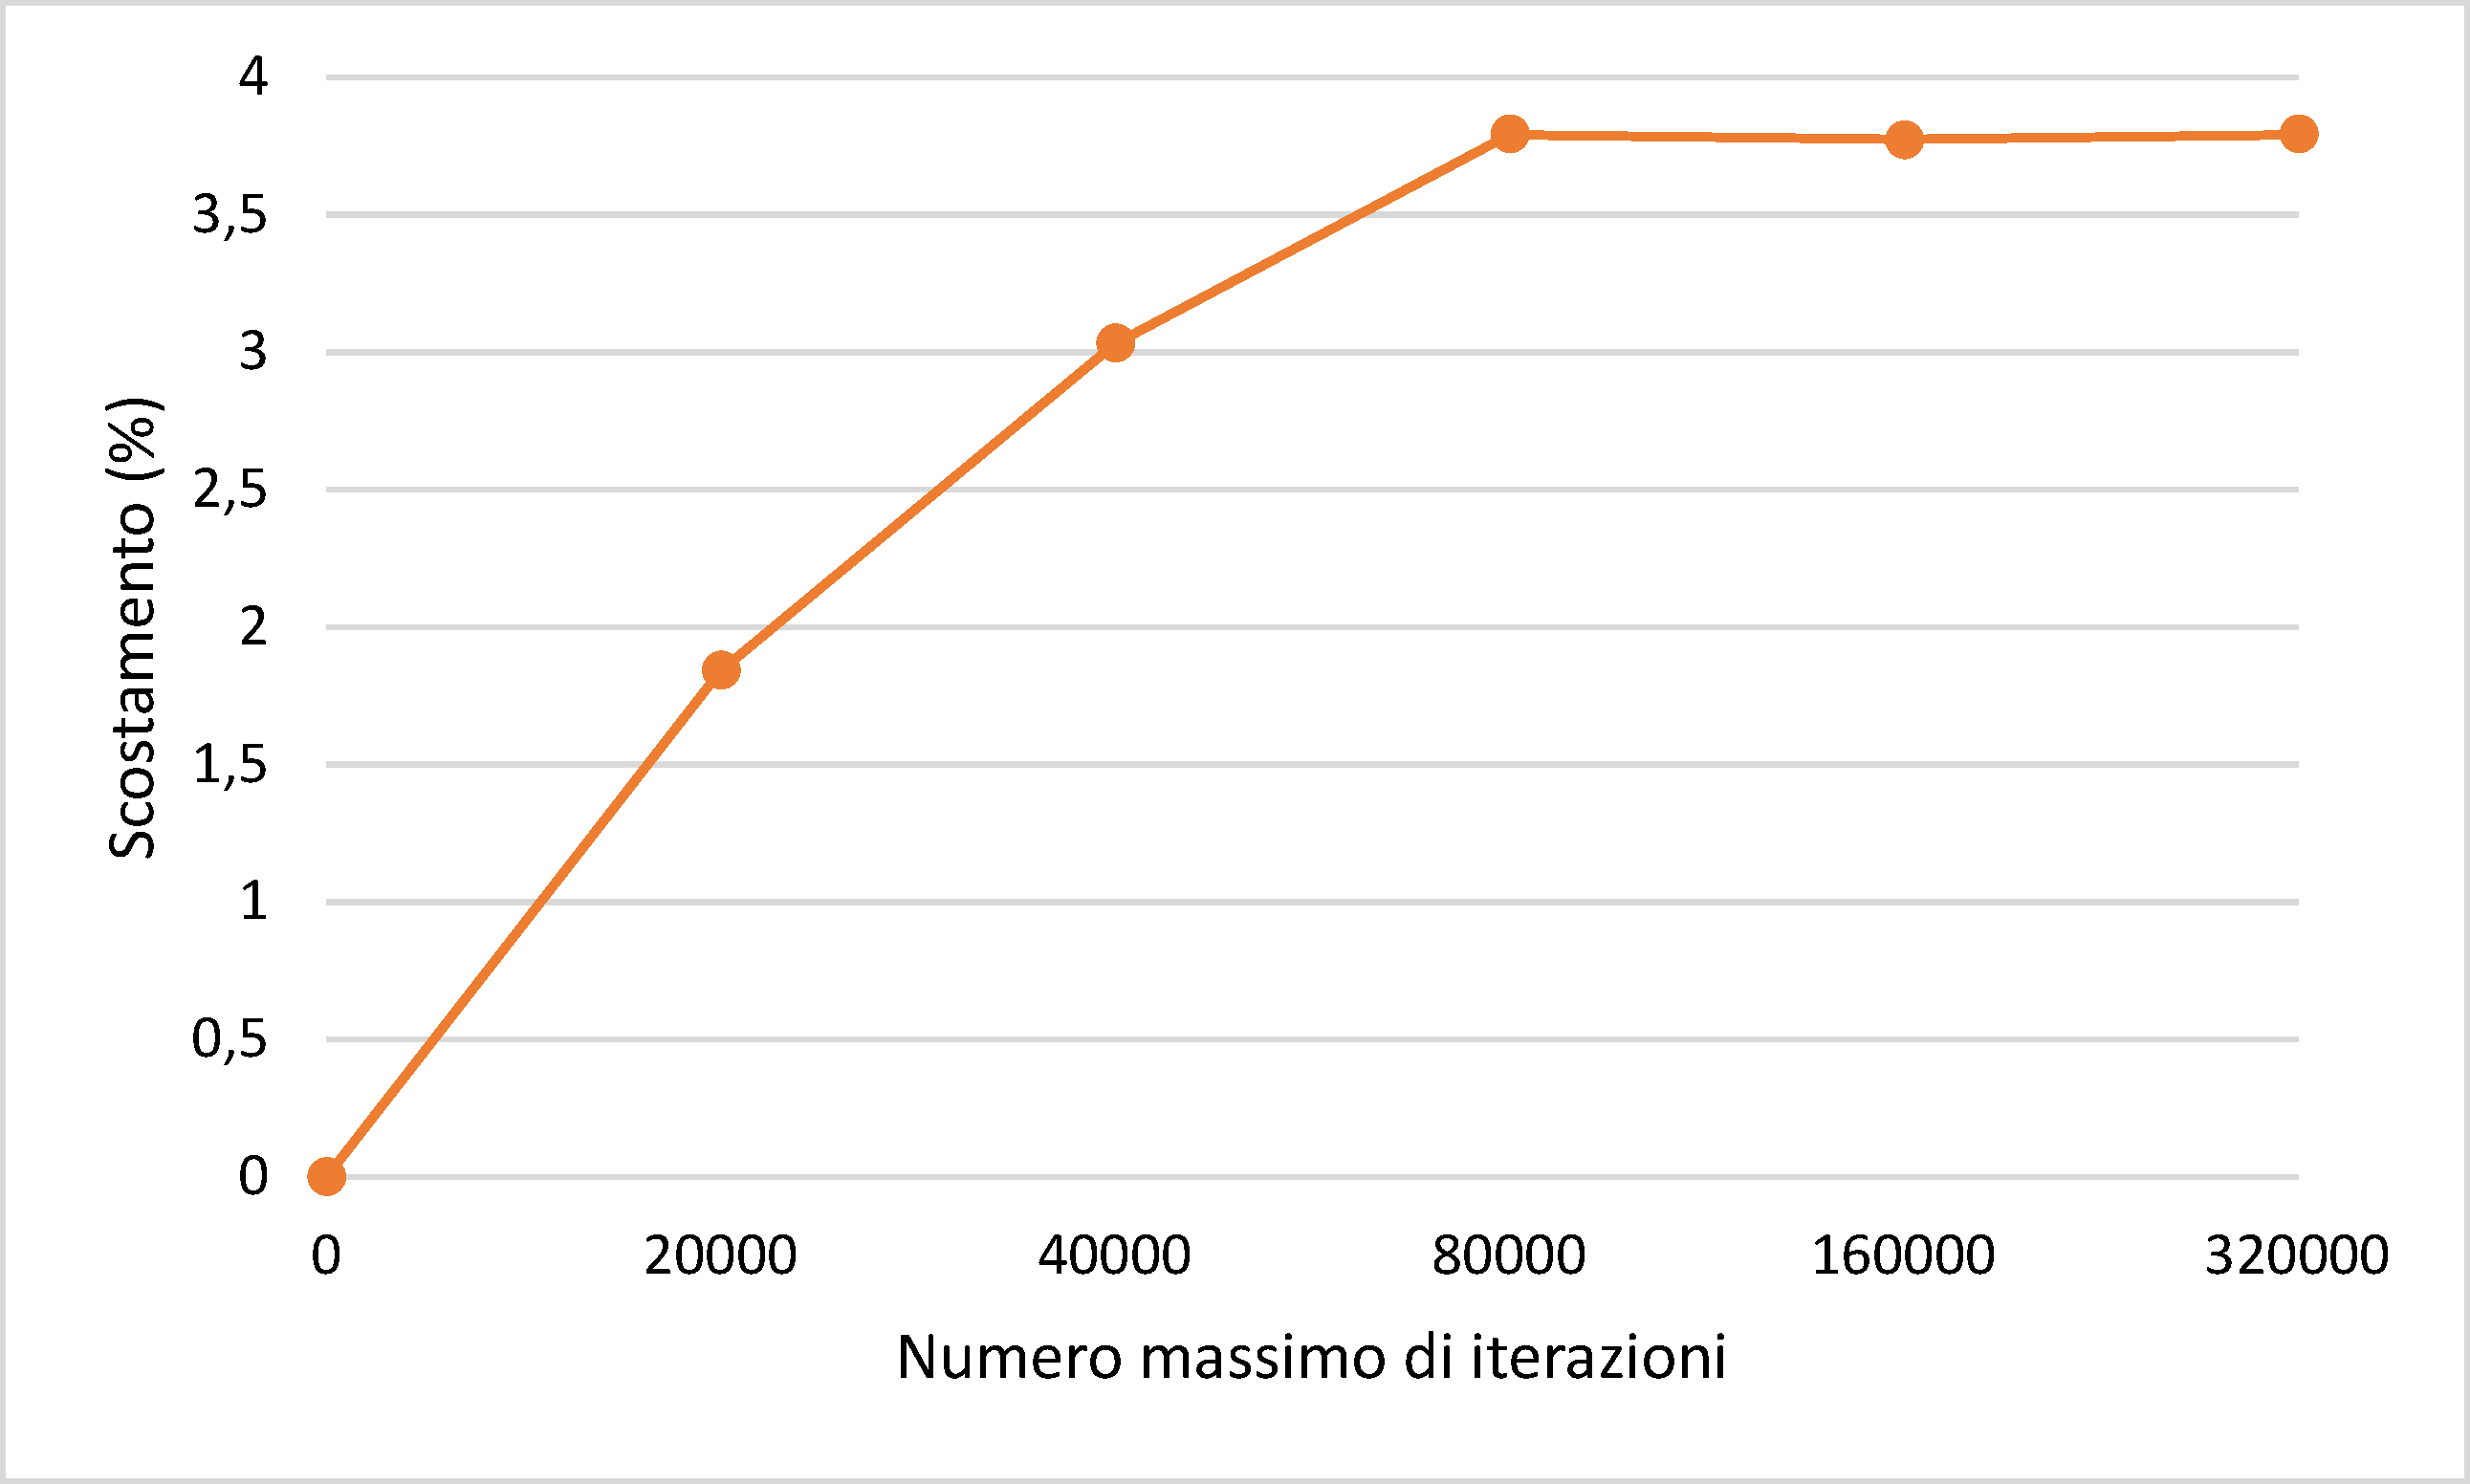
\includegraphics[scale=0.27]{risultati test/grafico max it.pdf}
    \caption{Grafico scostamento/iterazioni}
    \label{grafico-scostamento-iterazioni}
\end{figure}
\noindent Si osservino la Tabella \ref{tab:test-max-it} e la Figura \ref{grafico-scostamento-iterazioni}.
\noindent Nell'esempio, lo scostamento percentuale dei
totali inizialmente aumenta, per poi rimanere in stallo raggiunto un certo numero di iterazioni.\\
Questo potrebbe accadere poichè, molto probabilmente, si è raggiunto un buon minimo locale e dunque la probabilità
di trovare una mossa migliorante sarebbe molto bassa.\\[0.1cm]
\textbf{Confronto fra le scelte di risoluzione dei vincoli}\hfill\\[0.1cm]
Dati in \textit{input}:
\begin{itemize}
    \item tipo di inizializzazione: \textit{HighestArtRequestByArt}
    \item numero massimo di iterazioni: 20000
    \item numero massimo di iterazioni non miglioranti: 2500
    \item grandezza della \textit{Tabu list}: 200
    \item tempo di esecuzione massimo: 10 minuti (da requisito \hyperref[tab:requisiti-di-performance]{R45-P-O})
\end{itemize}

\begin{table}[!h]
    \centering
    \caption{\textit{Test} - scelta di risoluzione dei vincoli}
    \label{tab:test-risoluzione}
    \begin{tabular}{|c|c|c|c|}
    \hline
    \rowcolor{lighter-grayer}
    \textbf{Risoluzione} & \textbf{PreTot (€)} & \centering \textbf{PostTot (€)} & \centering \textbf{Scostamento (\%)} \arraybackslash \\
    \hline
    \textit{Min/Max} & \multirow{3}{*}{24.876,15} & 24.418,43 & 1,84 \arraybackslash \\ \cline{1-1} \cline{3-4}
    \valtest{Proporzionale}{24.465,69}{1,65}
    Ricompattamento & & 24.386,09 & 1,97 \arraybackslash \\ \hline
    \end{tabular}
\end{table}
\newpage
dove:
\begin{itemize}
    \item Risoluzione $=$ tipo di risoluzione dei vincoli;
    \item PreTot $=$ totale dell'ordine prima dell'operazione di ottimizzazione;
    \item PostTot $=$ totale dell'ordine dopo l'operazione di ottimizzazione;
    \item Scostamento $=$ scostamento percentuale fra $PreTot$ e $PostTot$.
\end{itemize}
\begin{figure}[!h] 
    \centering
    \vspace*{0.2cm}
    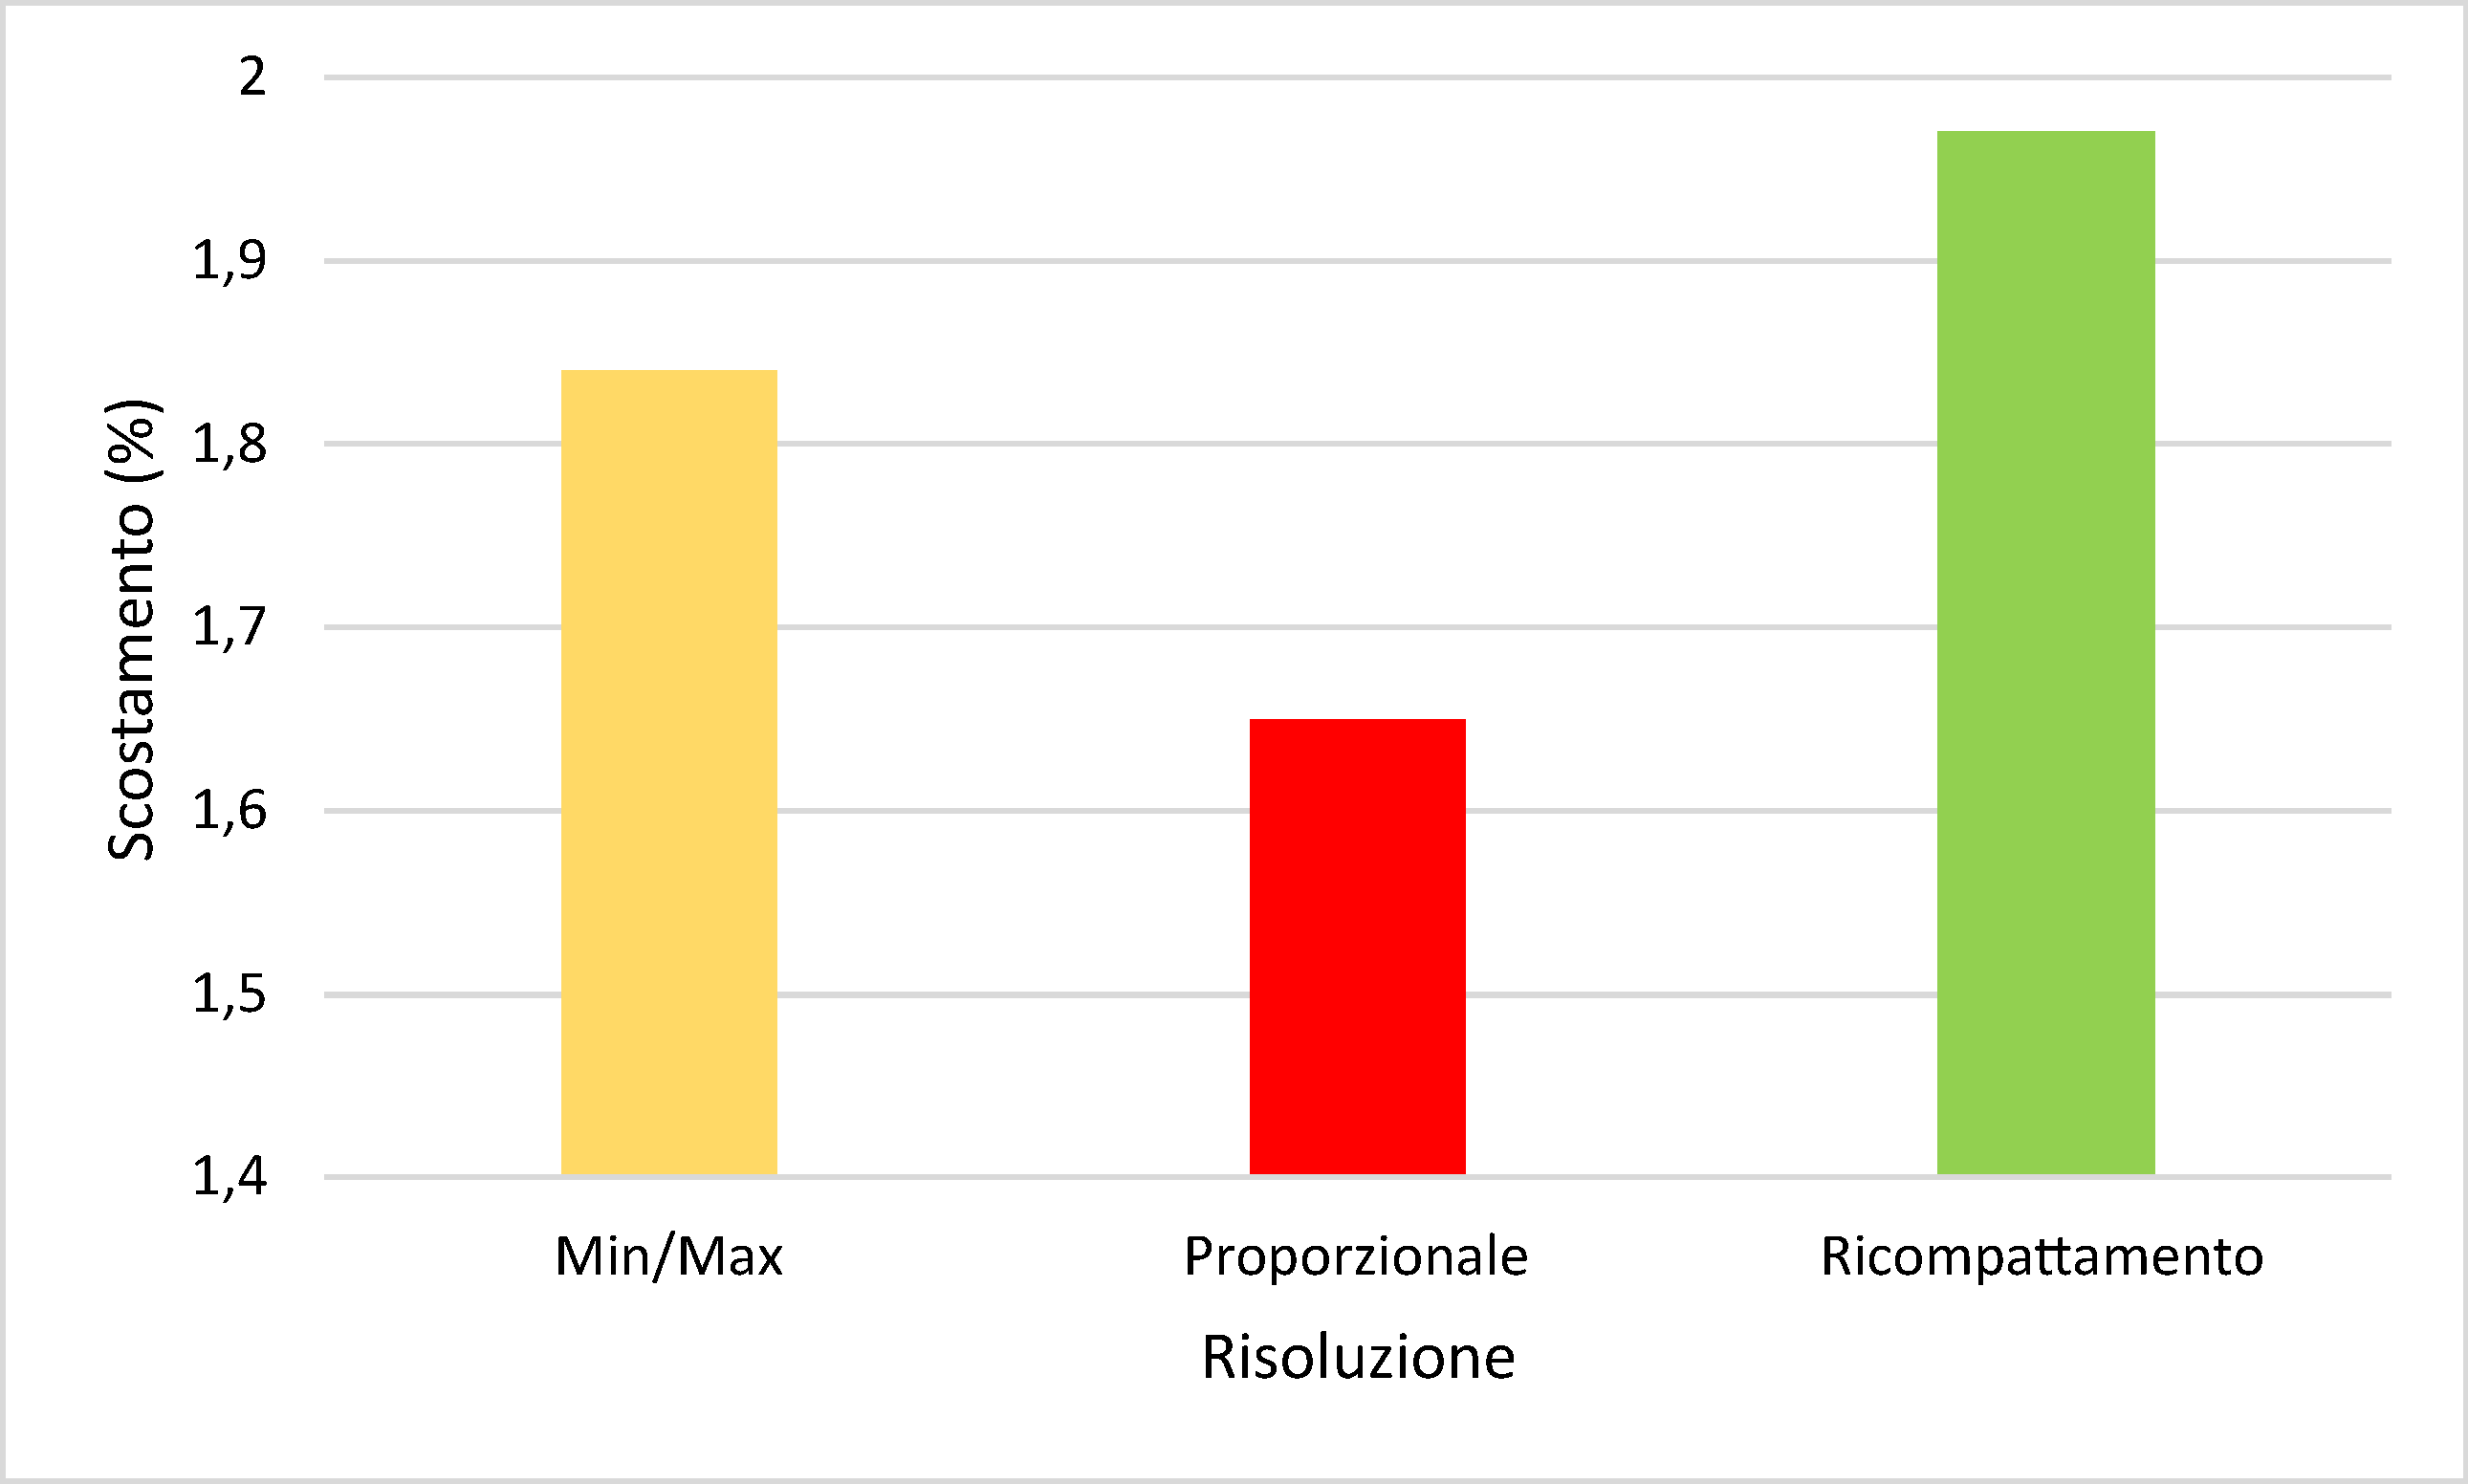
\includegraphics[scale=0.27]{risultati test/grafico risoluzione.pdf}
    \caption{Grafico scostamento/risoluzione}
    \label{grafico-scostamento-risoluzione}
\end{figure}
\noindent Si osservino la Tabella \ref{tab:test-risoluzione} e la Figura \ref{grafico-scostamento-risoluzione}.
Nell'esempio, l'utilizzo del metodo proporzionale sembrerebbe provocare lo scostamento minore di tutti.\\
Questo potrebbe indicare
che, nel controllo del minimo relativo
al singolo ordine, si potrebbe avere una più alta probabilità, rispetto agli altri metodi, di aumentare di una unità la quantità di un ordine
con prezzo unitario che non corrisponde al minimo.\\
\noindent Il ricompattamento, invece, sembrerebbe provocare lo scostamento maggiore di tutti.\\
Questo potrebbe succedere perchè la mossa è pensata per evitare di comprare
articoli in eccesso, andando così a ridurre le scorte di magazzino (e conseguentemente anche
il prezzo totale speso).\\